\documentclass{article}

\usepackage[margin=1.0in]{geometry}
\usepackage{graphicx}
\usepackage{amsmath}
\usepackage{float}
\usepackage{enumitem}

\title{CSC 535 HW6}
\date{10/31/2018}
\author{Simon Swenson}

\begin{document}

\pagenumbering{gobble}
\maketitle
\pagenumbering{arabic}

\large Introduction

\small I completed all required homework problems.

\section{Q1}

A table with the distribution of the measured angles (columns), given an angle 
(rows).

\begin{tabular}{r | c c c c c c c c c}
      & 1   & 2   & 3   & 4   & 5   & 6   & 7   & 8   & 9   \\
    1 & 0.7 & 0.2 & 0.1 & 0   & 0   & 0   & 0   & 0   & 0   \\
    2 & 0.3 & 0.4 & 0.2 & 0.1 & 0   & 0   & 0   & 0   & 0   \\
    3 & 0.1 & 0.2 & 0.4 & 0.2 & 0.1 & 0   & 0   & 0   & 0   \\
    4 & 0   & 0.1 & 0.2 & 0.4 & 0.2 & 0.1 & 0   & 0   & 0   \\
    5 & 0   & 0   & 0.1 & 0.2 & 0.4 & 0.2 & 0.1 & 0   & 0   \\
    6 & 0   & 0   & 0   & 0.1 & 0.2 & 0.4 & 0.2 & 0.1 & 0   \\
    7 & 0   & 0   & 0   & 0   & 0.1 & 0.2 & 0.4 & 0.2 & 0.1 \\
    8 & 0   & 0   & 0   & 0   & 0   & 0.1 & 0.2 & 0.4 & 0.3 \\
    9 & 0   & 0   & 0   & 0   & 0   & 0   & 0.1 & 0.2 & 0.7 \\
\end{tabular}

The distributions are not the same because of the squishing effects at the ends.
The variance will be much less at the ends as a result.

\section{Q2}

\begin{figure}[!ht]
	\centering
	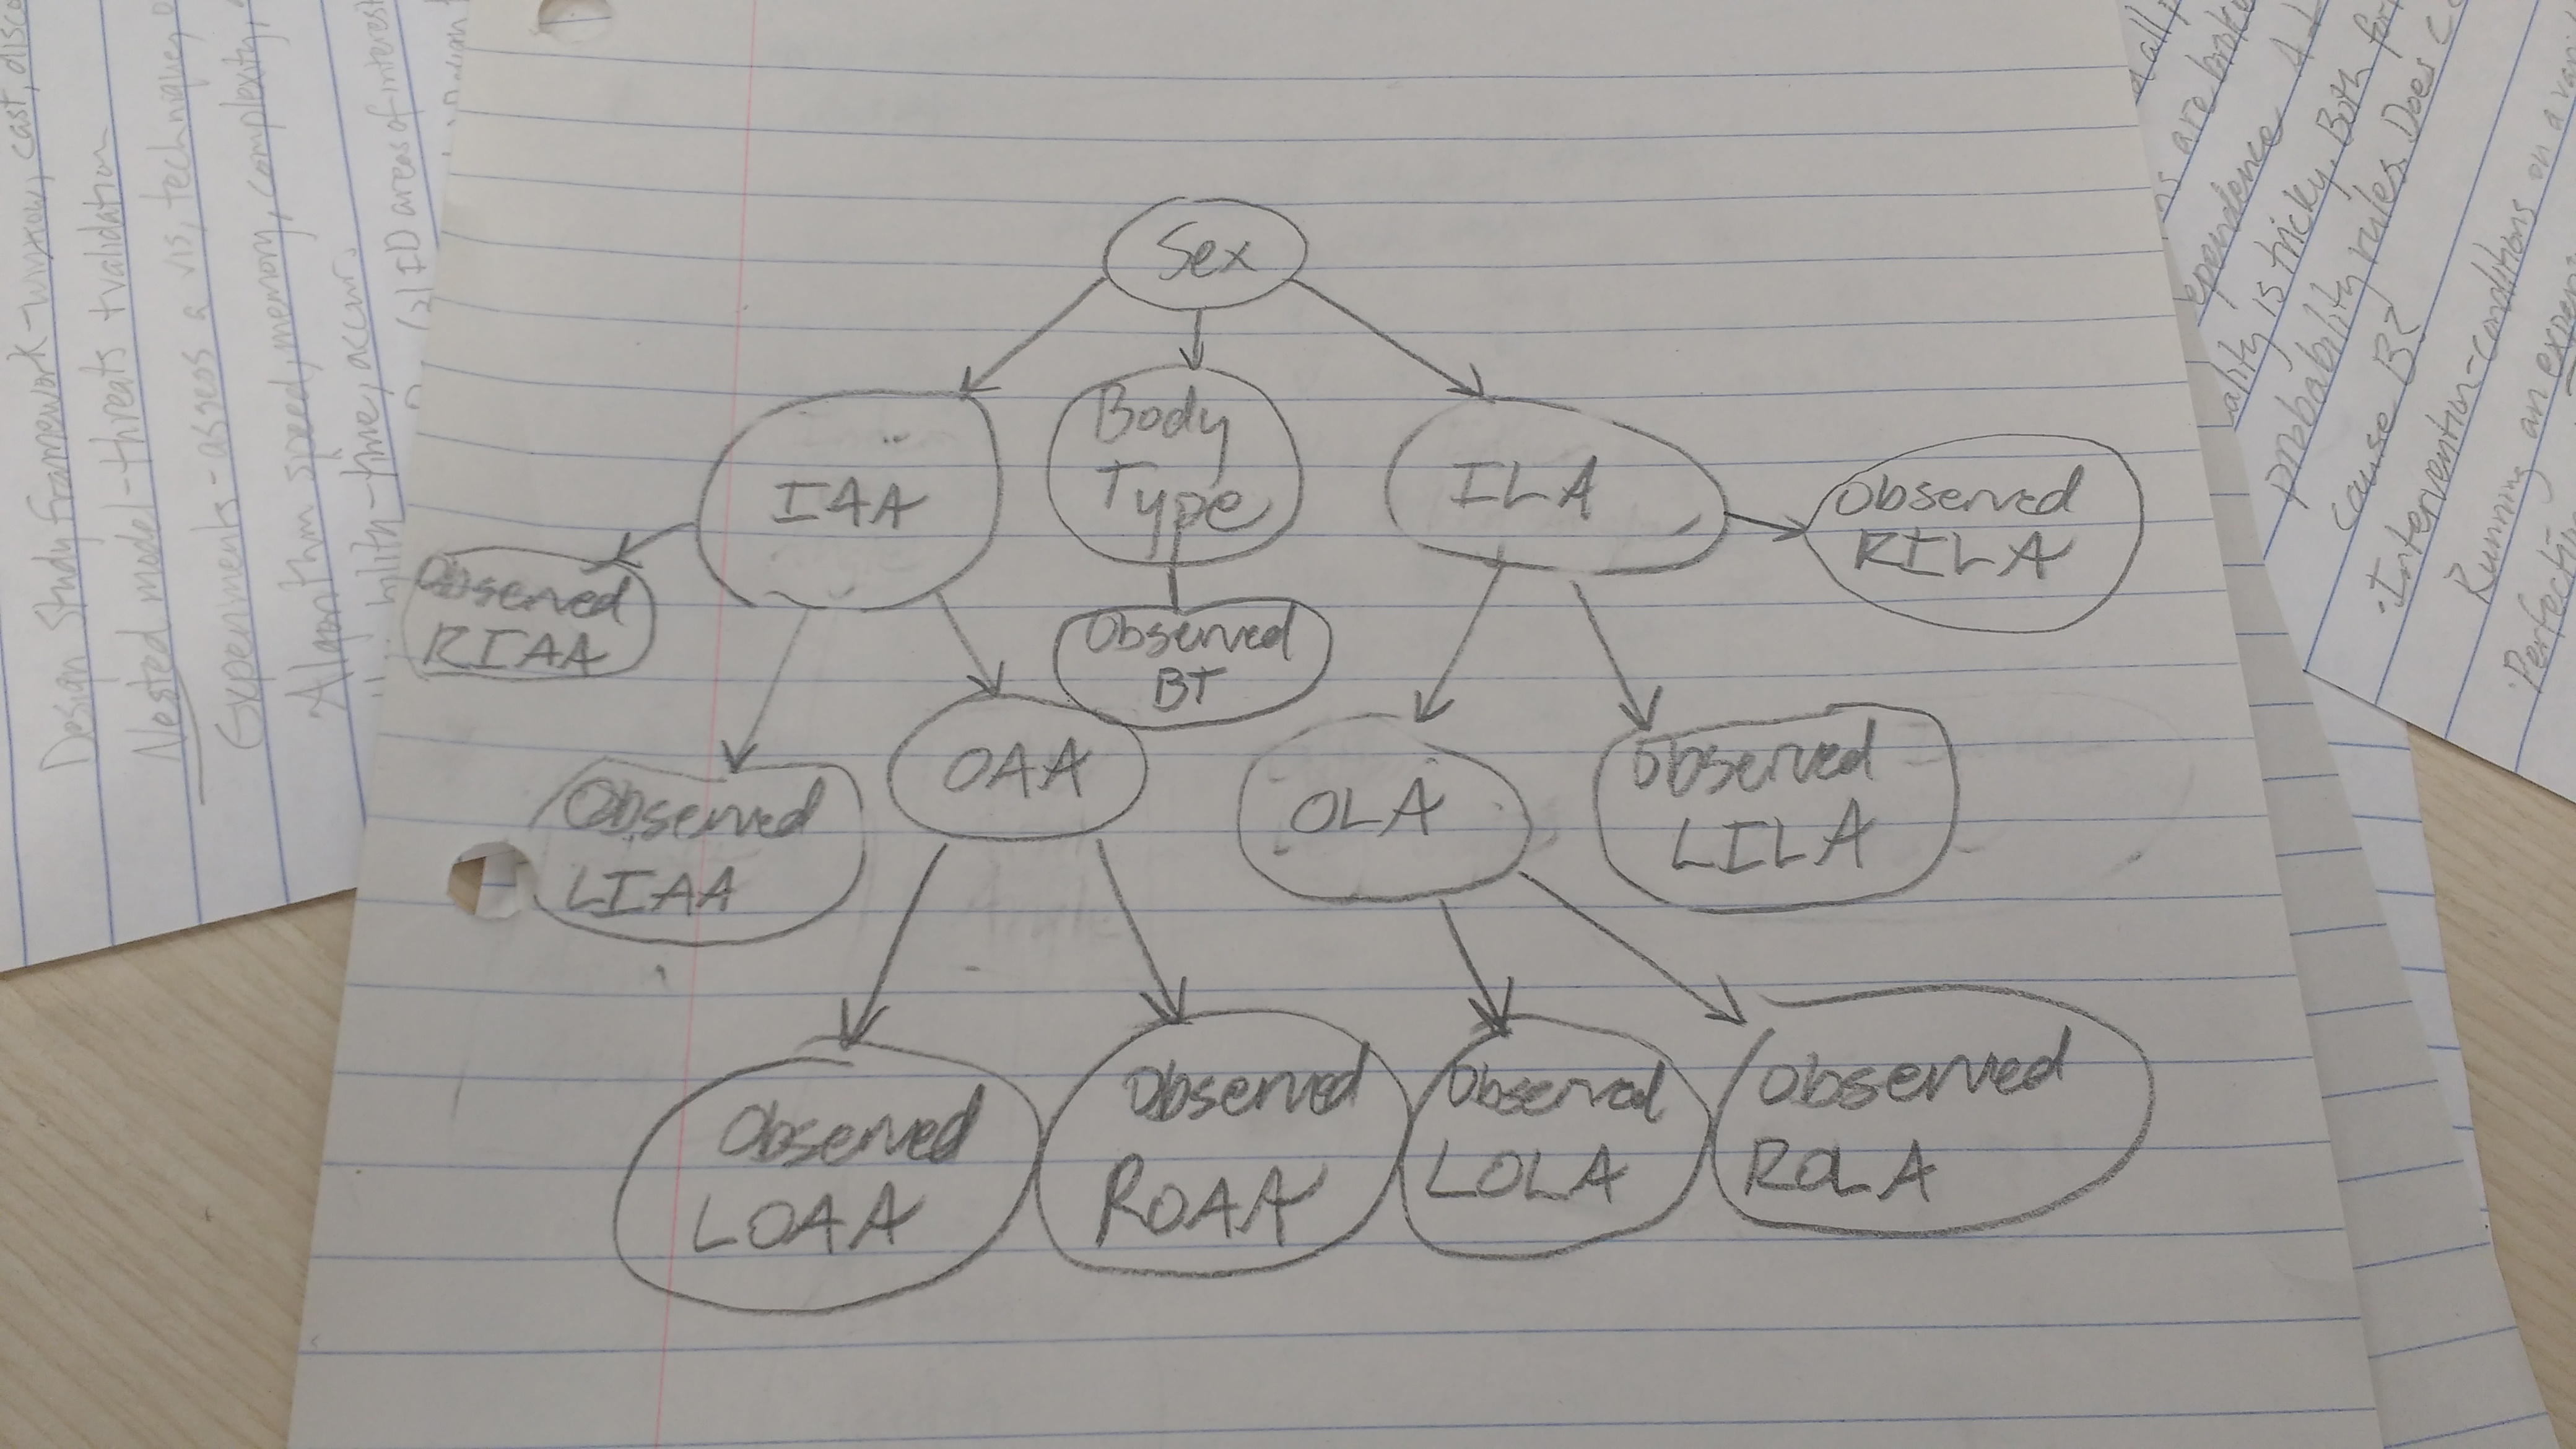
\includegraphics[width=120mm]{figs/mql-pgm.jpg}
	\caption{The corresponding directed Bayes's net for the distribution 
        discribed in the homework assignment.}
\end{figure}

\section{Q3}

$$
P(S, BT, IAA, ILA, OBT, OLIAA, ORIAA, OAA, OLA, OLILA, ORILA, OLOAA, OROAA, OLOLA, OROLA) =
$$ $$
P(S) P(BT | S) P(IAA | S) P(ILA | S) P(OBT | BT) P(OLIAA | IAA) P(ORIAA | IAA)
$$ $$
P(OAA | IAA) P(OLA | ILA) P(OLILA | ILA) P(ORILA | ILA) P(OLOAA | OAA)
$$ $$
P(OROAA | OAA) P(OLOLA | OLA) P(OROLA | OLA)
$$

\section{Q4}

\begin{figure}[!ht]
	\centering
	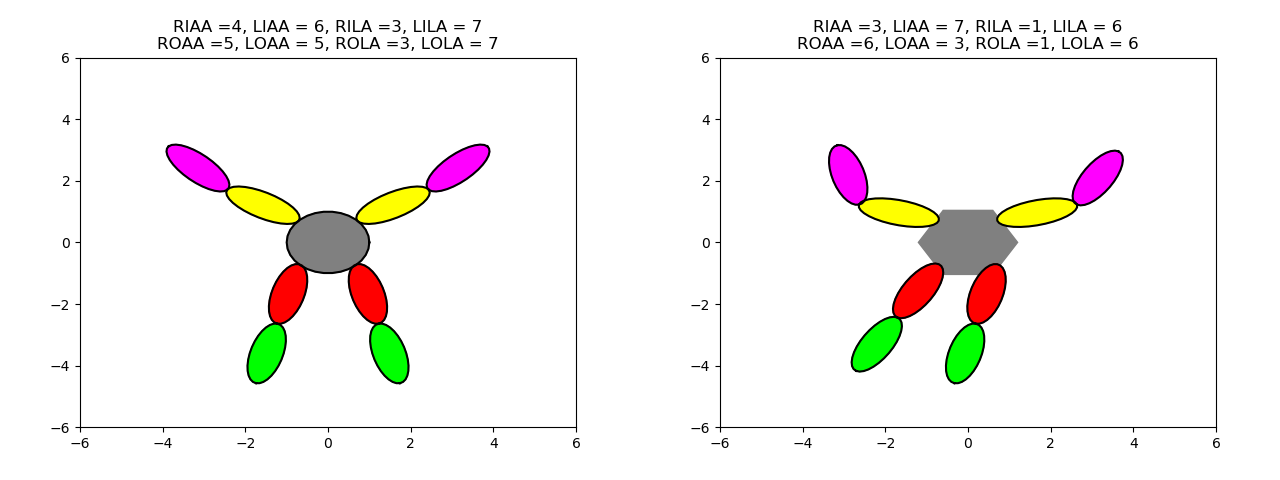
\includegraphics[width=120mm]{figs/mql-1.png}
	\caption{Actual (left) and observed (right) measurements for magnetic-quad-limb one.}
\end{figure}
\begin{figure}[!ht]
	\centering
	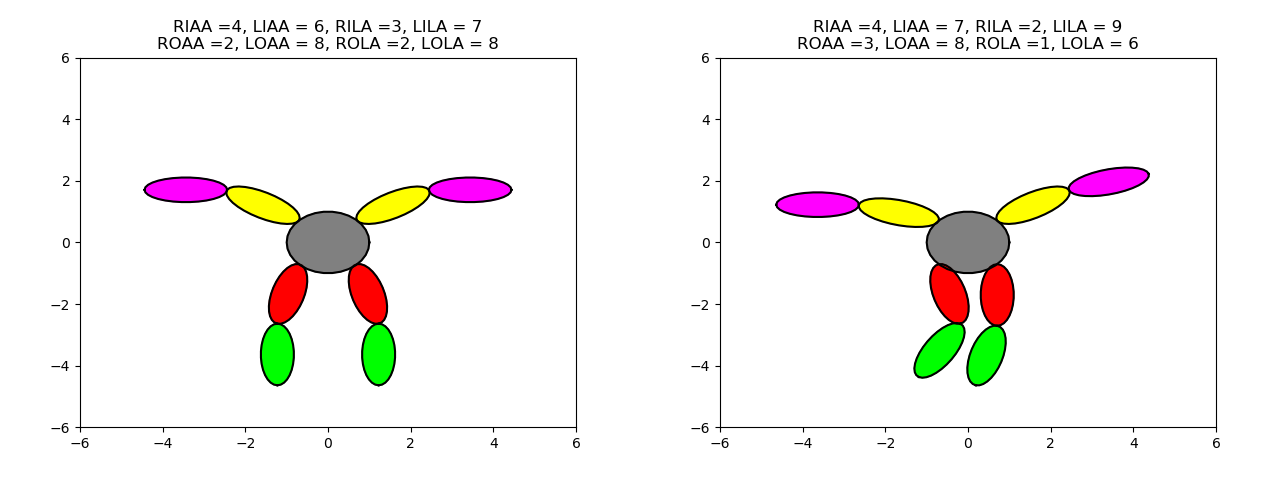
\includegraphics[width=120mm]{figs/mql-2.png}
	\caption{Actual (left) and observed (right) measurements for magnetic-quad-limb two.}
\end{figure}
\begin{figure}[!ht]
	\centering
	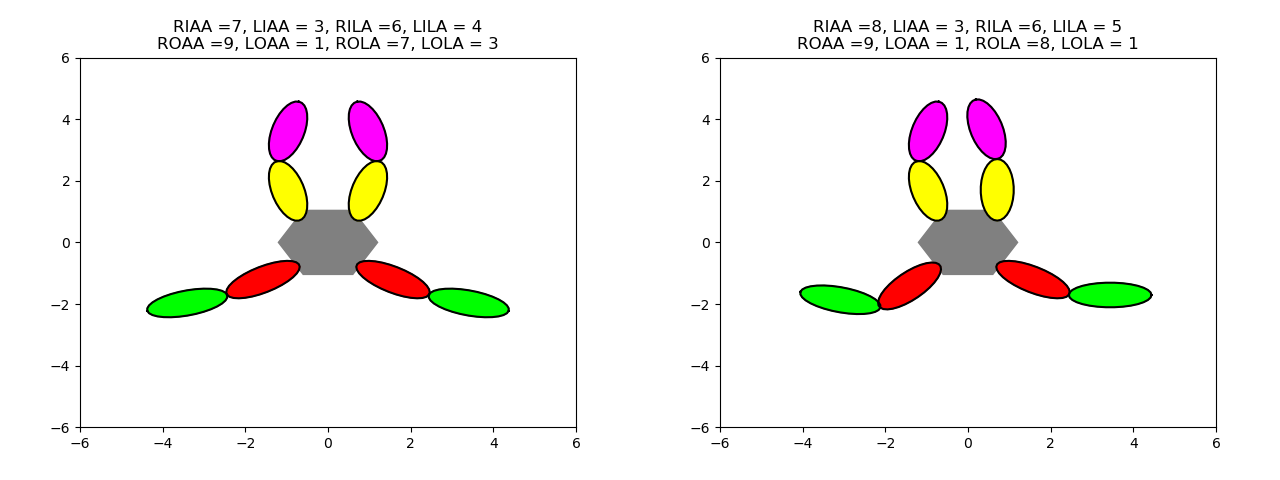
\includegraphics[width=120mm]{figs/mql-3.png}
	\caption{Actual (left) and observed (right) measurements for magnetic-quad-limb three.}
\end{figure}
\begin{figure}[!ht]
	\centering
	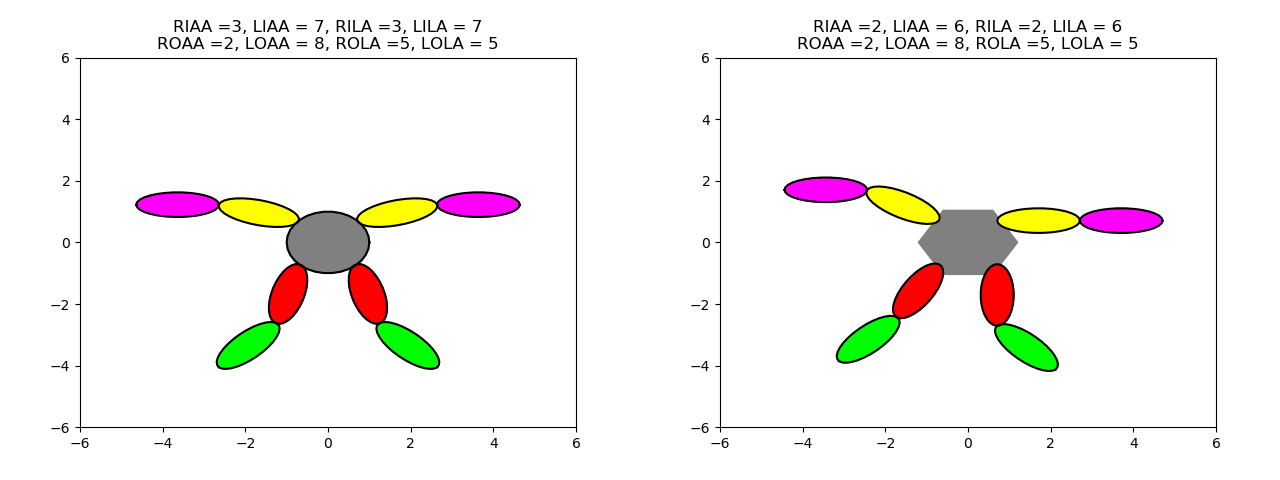
\includegraphics[width=120mm]{figs/mql-4.png}
	\caption{Actual (left) and observed (right) measurements for magnetic-quad-limb four.}
\end{figure}
\begin{figure}[!ht]
	\centering
	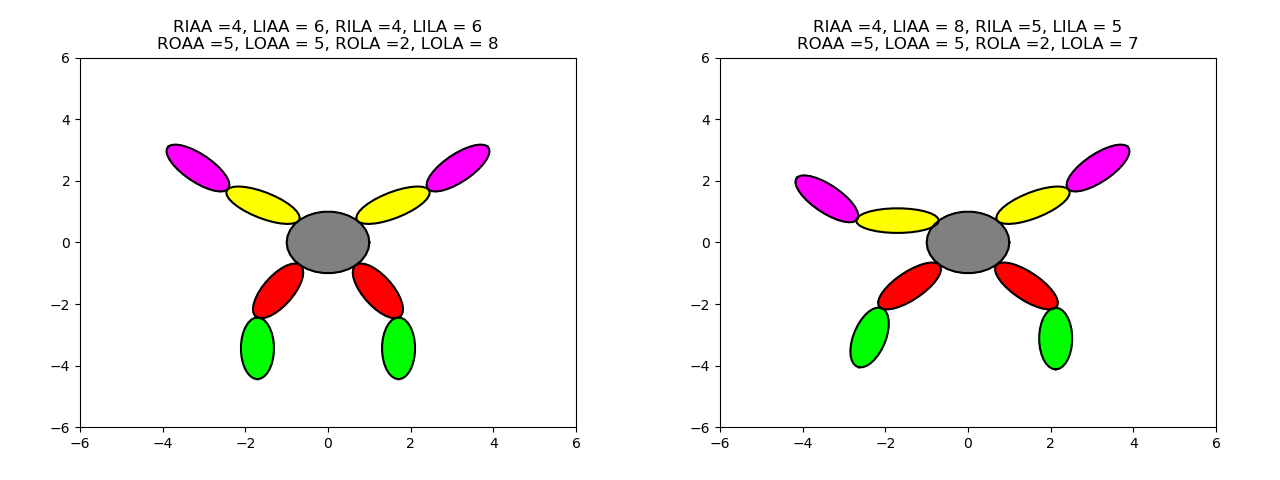
\includegraphics[width=120mm]{figs/mql-5.png}
	\caption{Actual (left) and observed (right) measurements for magnetic-quad-limb five.}
\end{figure}
\begin{figure}[!ht]
	\centering
	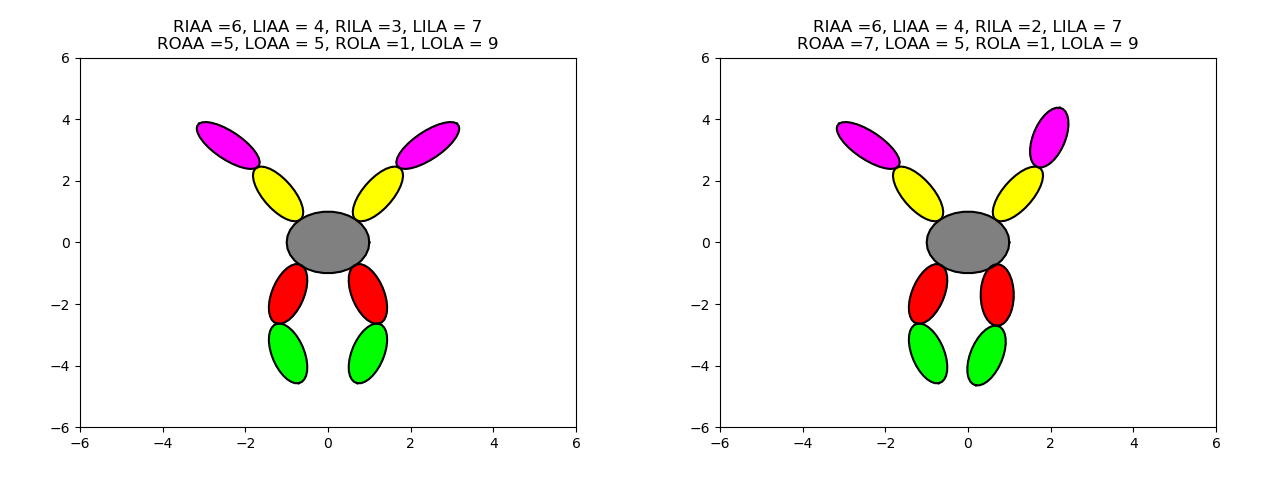
\includegraphics[width=120mm]{figs/mql-6.png}
	\caption{Actual (left) and observed (right) measurements for magnetic-quad-limb six.}
\end{figure}
\begin{figure}[!ht]
	\centering
	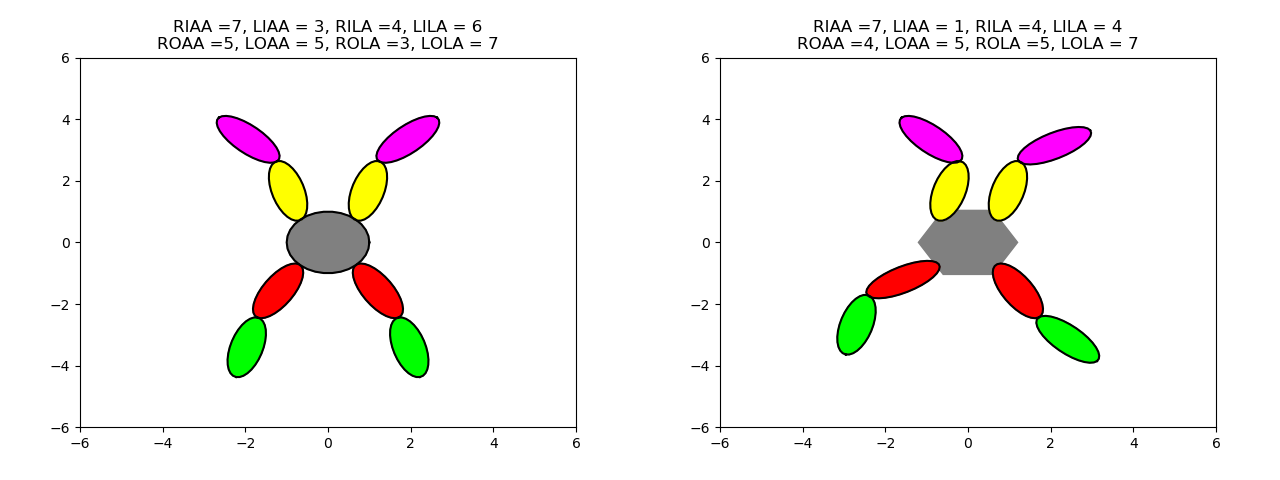
\includegraphics[width=120mm]{figs/mql-7.png}
	\caption{Actual (left) and observed (right) measurements for magnetic-quad-limb seven.}
\end{figure}
\begin{figure}[!ht]
	\centering
	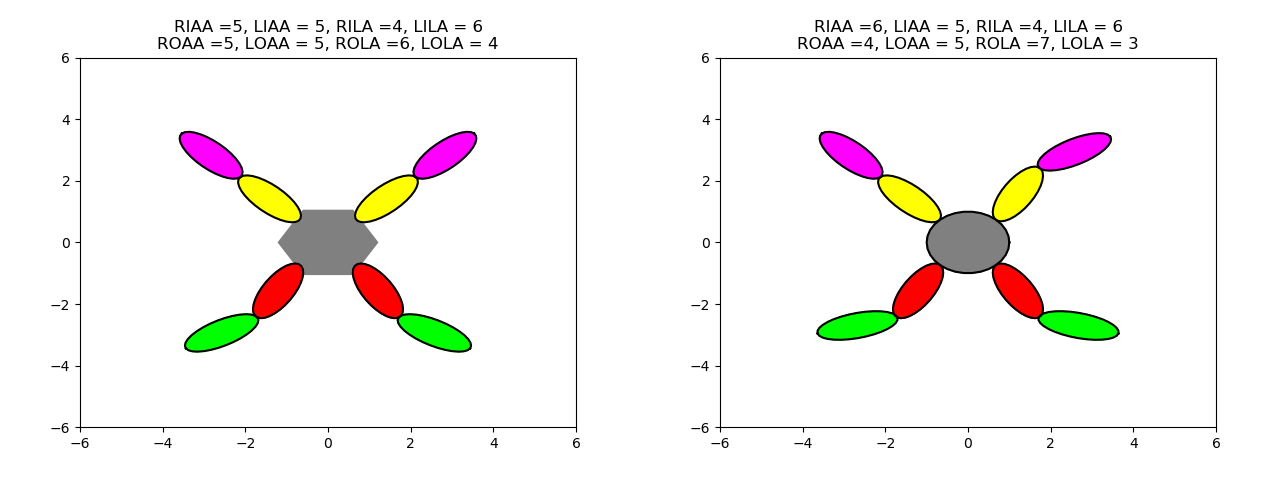
\includegraphics[width=120mm]{figs/mql-8.png}
	\caption{Actual (left) and observed (right) measurements for magnetic-quad-limb eight.}
\end{figure}
\begin{figure}[!ht]
	\centering
	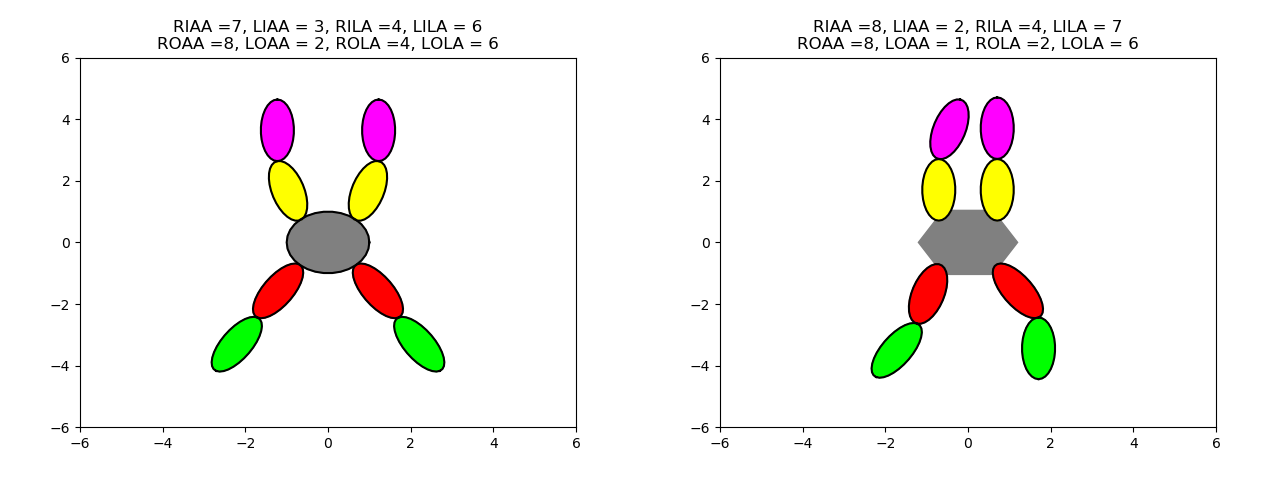
\includegraphics[width=120mm]{figs/mql-9.png}
	\caption{Actual (left) and observed (right) measurements for magnetic-quad-limb nine.}
\end{figure}
\begin{figure}[!ht]
	\centering
	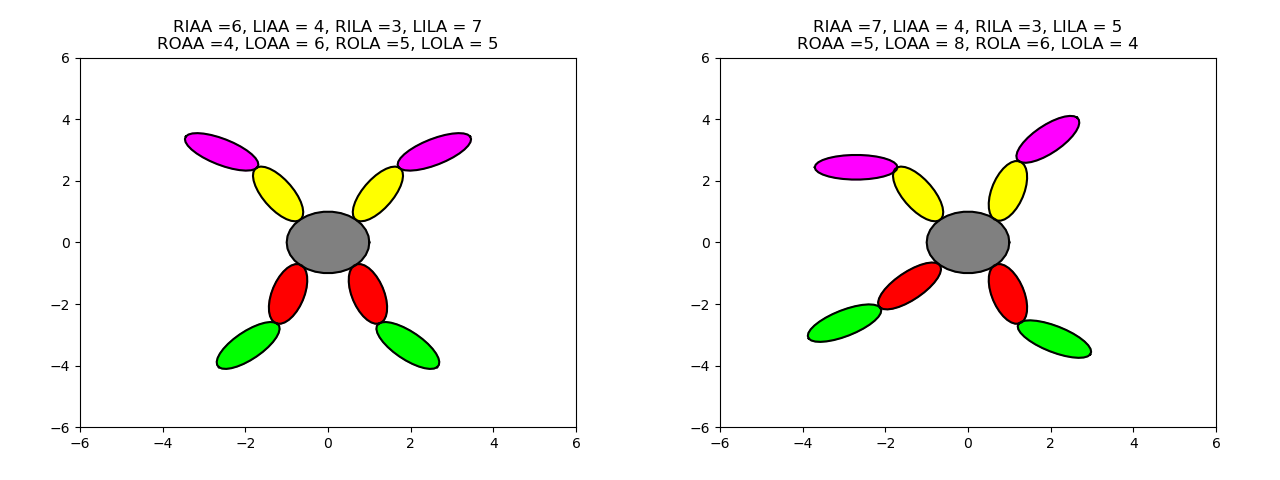
\includegraphics[width=120mm]{figs/mql-10.png}
	\caption{Actual (left) and observed (right) measurements for magnetic-quad-limb ten.}
\end{figure}

~\\
~\\
~\\
~\\
~\\
~\\
~\\
~\\
~\\
~\\
~\\
~\\
~\\
~\\
~\\
~\\
~\\
~\\
~\\
~\\
~\\
~\\
~\\

\section{Q5}

Our guesses and the degree of our the certainty of those guesses relies heavily 
on the underlying distributions. The distributions can give us clues about what 
sex is more likely, given a certain configuration. Some distributions are 
heavily skewed to one or two values. For example, $P(RILA = 3 | S = M) = 50/90$ 
whereas $P(RILA = 3 | S = F) = 10/90$, so, given an inner leg angle 
configuration of 3, the sex is much more likely to be male. Even with the 
uncertainty of the observed values, this can be relied on to skew our guess 
toward one sex or another. The other distributions also give us clues, and the 
degree to which those clues affect our guess is determined by how skewed the 
distributions are.

\end{document}